\documentclass{template/socthesis}

\usepackage{subcaption} 
\usepackage{amsmath} 
\usepackage{enumitem} 
\usepackage{hyperref} % reference
\usepackage{gensymb} % balíček symbolů
\usepackage{booktabs}

\usepackage[toc,page]{appendix}
\usepackage{color} % balíček pro obarvování textů
\usepackage{xcolor}  % zapne možnost používání barev, mj. pro \definecolor
\definecolor{mygreen}{RGB}{0,150,0} % nastavení barev odkazů 
\usepackage{listings} % balíček pro formátování zdrojových kódů 
\usepackage{multirow}
\usepackage{pifont}
\usepackage{pdfpages}
\usepackage{parskip}
\usepackage[author=,status=draft]{fixme} % vkládání poznámek  
% dva módy (status): draft (poznámky se zobrazují v~PDF) / final (poznámky se nezobrazují v~PDF)

\newcommand{\cmark}{\textcolor{green}{\ding{51}}}%
\newcommand{\xmark}{\textcolor{red}{\ding{55}}}%



\lstset { %
    language=C++,
    backgroundcolor=\color{black!5}, % set backgroundcolor
    basicstyle=\footnotesize,% basic font setting
}

\setlist[itemize]{parsep=1pt}

\addbibresource{text.bib} % soubor s~bibliografií
\nocite{*}


% hinty k~používání balíčků hyperref, url, hyperlink a~hypertarget
% \usepackage{hyperref} % balíček pro hypertextové odkazy
% \url{www.odkaz.cz}
% \href{http://www.odkaz.cz}{Text který bude jako odkaz}
% \hyperlink{label}{proklikávací_text} - odkaz na text 
% \hypertarget{label}{cíl_odkazu} - cíl odkazu 

\begin{document} % konec preambule dokumentu


% #########################################################################################
\chapter{Abstrakt}

Cílem mé práce bylo navrhnout ucelený automatický systém monitorující chod pletacích strojů a~přizpůsobit ho co možná nejlépe potřebám výrobní firmy.

Systém jsem navrhoval na míru pro rodinnou firmu na pletení ponožek a~v sou\-čas\-nos\-ti je schopen v~reálném čase zaznamenávat a~následně odesílat naměřená data ze strojů na server. 
Pro uživatele systém nabízí moderní webové stránky, kde si může naměřená data přehledně zobrazit a~analyzovat.

Systém se skládá ze senzorové části, serveru a podpůrného serveru.
Senzorová část je připojená k~pletacímu stroji a~odesílá naměřená data.
Server zajišťuje veškeré zpracování dat a jejich zobrazení uživateli.
Podpůrný server se stará o~aktualizaci a~o~kontrolu správného chodu senzorů.


% #########################################################################################
\chapter{Synopse}

\section{Úvod}
Práce s názvem Integrace do průmyslu 4.0 se zabývá návrhem monitorovacího systému pro firmu na výrobu ponožek.
Celý systém je nasazen v rodinné firmě ROTEX Vysočina \cite{ROTEX}, která pracuje ve dvousměnném provozu a produkuje měsíčně přes dvanáct tisíc párů ponožek.

Ve firmě je 25 pletacích strojů na ponožky o které se v každé směně starají tři operátoři.
Samotná práce operátora spočívá v kontrole upletených vzorků, otáčení dopletených ponožek a opravách porouchaných strojů.

Můj systém, který jsem interně pojmenoval Pletačka IoT, se stará o monitoring počtu upletených ponožek, dobu zastavení jednotlivých strojů, porovnávání jednotlivých směn, ale také dává zaměstnavateli přehled o aktuální produkci.

\begin{figure}[htbp]
    \centering
    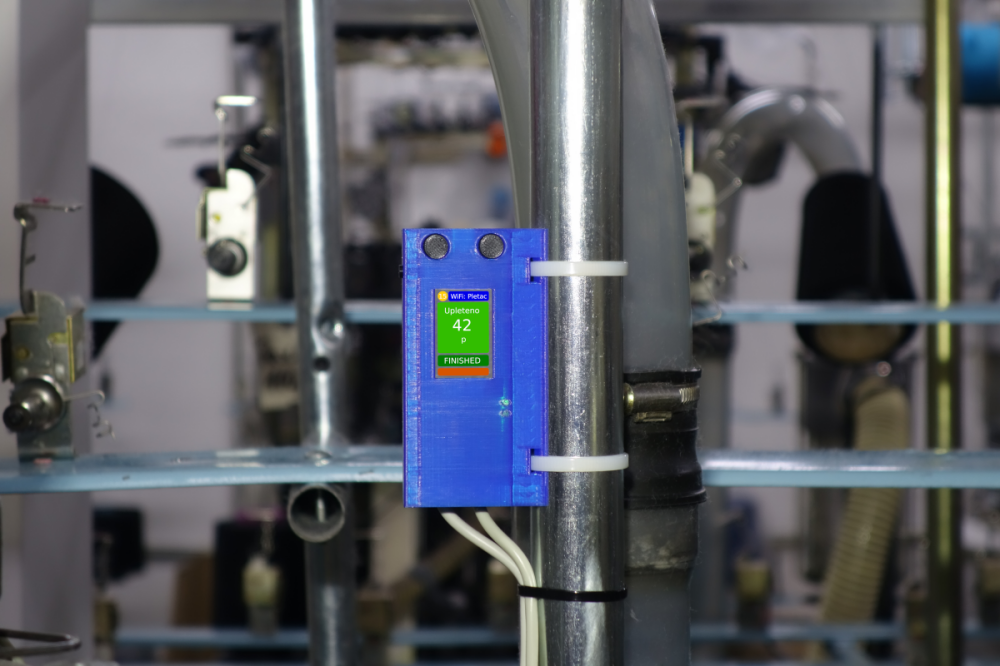
\includegraphics[width=\textwidth]{img/V2-uchyceni.png}
    \caption{Senzor na stroji}
    \label{fig:SenzorNaStroji}
\end{figure}


% #########################################################################################
\section{Senzory}

Na každém pletacím stroji je namontován jeden bezdrátový senzor, který odesílá data na server.
Pletací stroje jsou obvyklá průmyslová zařízení k jednomu účelu, čili pletení ponožek.
S příchodem modernizace průmyslových výroben se začíná více brát ohled na reálnou produkci a její automatizovaný monitoring.
Senzory Pletačka IoT jsem navrhoval tak, aby se daly jednoduše připojit na stávající pletací stroje a napojit je tak do centrálního řídícího systému.
Dalším požadavkem senzoru bylo, aby neohrožoval chod samotného stroje, pokud tedy není můj systém aktivní, nemá to žádný vliv na chod firmy.

Senzory jsou postavené na mikrokontroléru ESP32, který nabízí dostatečný výkon a má bezdrátovou konektivitu WiFi.
Každý z~těchto senzorů má svoje jedinečné číslo pod kterým posílá naměřená data na server.
Senzor je napájen z~5 nebo 24~V~a~má spotřebu 120 mA.

\begin{figure}[htbp]
    \centering
    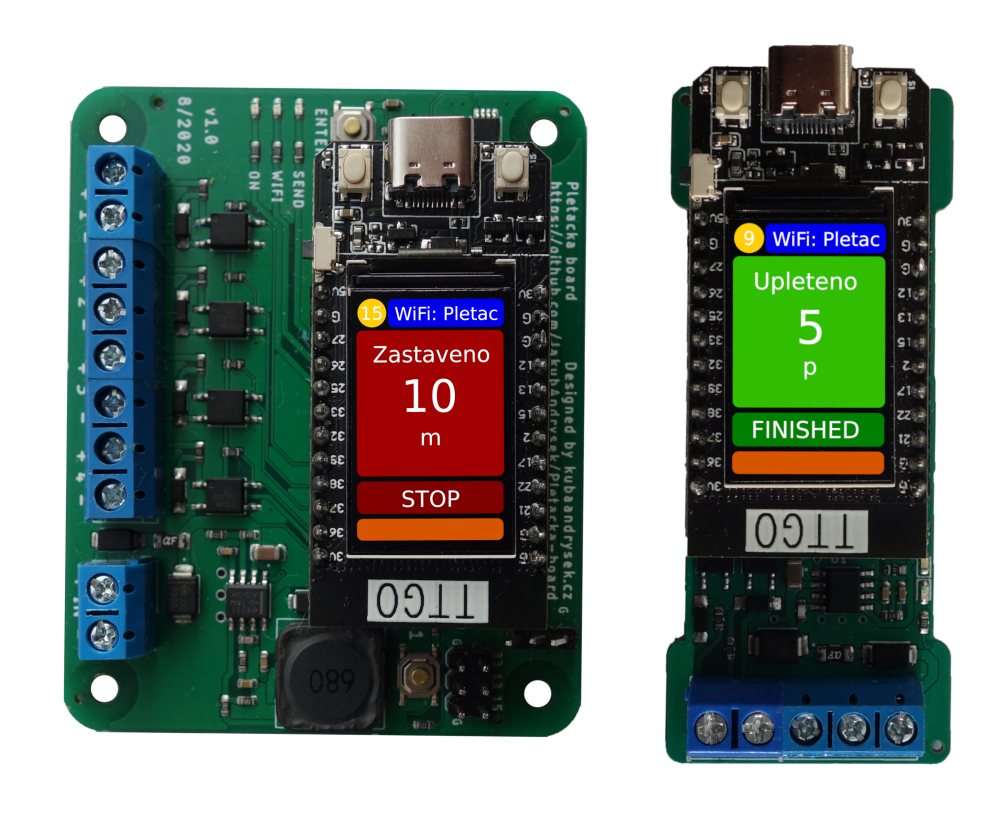
\includegraphics[width=\textwidth]{img/oba.png}
    \caption{Senzor na stroji}
    \label{fig:SenzorNaStroji}
\end{figure}

Na každém senzoru jsou dva optočleny napojené na indikační diody pletacího stroje.
Z jedné diody se snímá zastavení stroje pro výpočet poruchového času a z druhé senzor získává počet upletených ponožek.
Na těchto dvou údajích je postavený celý měřící a výpočetní systém.
Dále senzor obsahuje dvě uživatelská tlačítka sloužící pro nastavení jedinečného ID senzoru.
Pro rychlé grafické znázornění jsou na desce také dvě barevné diody.

Hlavní vizuální roli zajišťuje LCD displej, na kterém se operátorům zobrazují základní údaje o stroji.
Ve vrchní části jsou vypsány údaje o bezdrátovém připojení a číslo senzoru.
Uprostřed se operátorovi velkým písmem zobrazuje počet upletených ponožek a v případně zastavení stroje čas odstávky.
Tyto údaje se na každém stroji výrazně vykreslují a upozorňují tak obsluhu k brzké opravě.
Poslední novinku, kterou jsem na senzory doprogramoval je zobrazování průměrné rychlosti pletení ponožek za hodinu.
S takovýmto typem rychlosti se každodenně setkáváme například v autě a operátor z ní dokáže rychle dopočítat čas dopletení zakázky. 


% #########################################################################################
\section{Webový server}

Nedílnou součástí tohoto systému je také serverová část, která se stará o přijímání naměřených dat, jejich zpracování a následné zobrazení uživateli.
Samotný server běží na mikropočítači Raspberry Pi~4 Modelu~B.

Na zařízení běží operační systém Raspberry Pi OS s~grafickým rozhraním.
Webové stránky běží na HTTP serveru Apache2 a~PHP~8.0.
Jako databázový systém využívám MariaDB.
Server běží lokálně uvnitř firmy v~zabezpečené síti, díky čemuž je systém rychlý a~nezávislý na internetovém připojení.

Na webový server se dá jednoduše připojit otevřením lokálního firemního odkazu \href{http://pletacka.local}{pletacka.local}.
Poté se uživateli zobrazí úvodní přehledová stránka s barevnými bublinami, které představují jednotlivé pletací stroje.
Jejich barva pak udává v jakém stavu se stroj aktuálně nachází. Uživatel tak dokáže velmi rychle zjístit aktuální funkčnost pletacích strojů bez nutnosti návštěvy pletárny.
Kromě barvy se v bublině zobrazuje také text, ten ukazuje počet upletených ponožek aktuální směnu a v případě zastavení stroje a zčervenání se text změní na dobu zastavení stroje.

\begin{figure}[htbp]
    \centering
    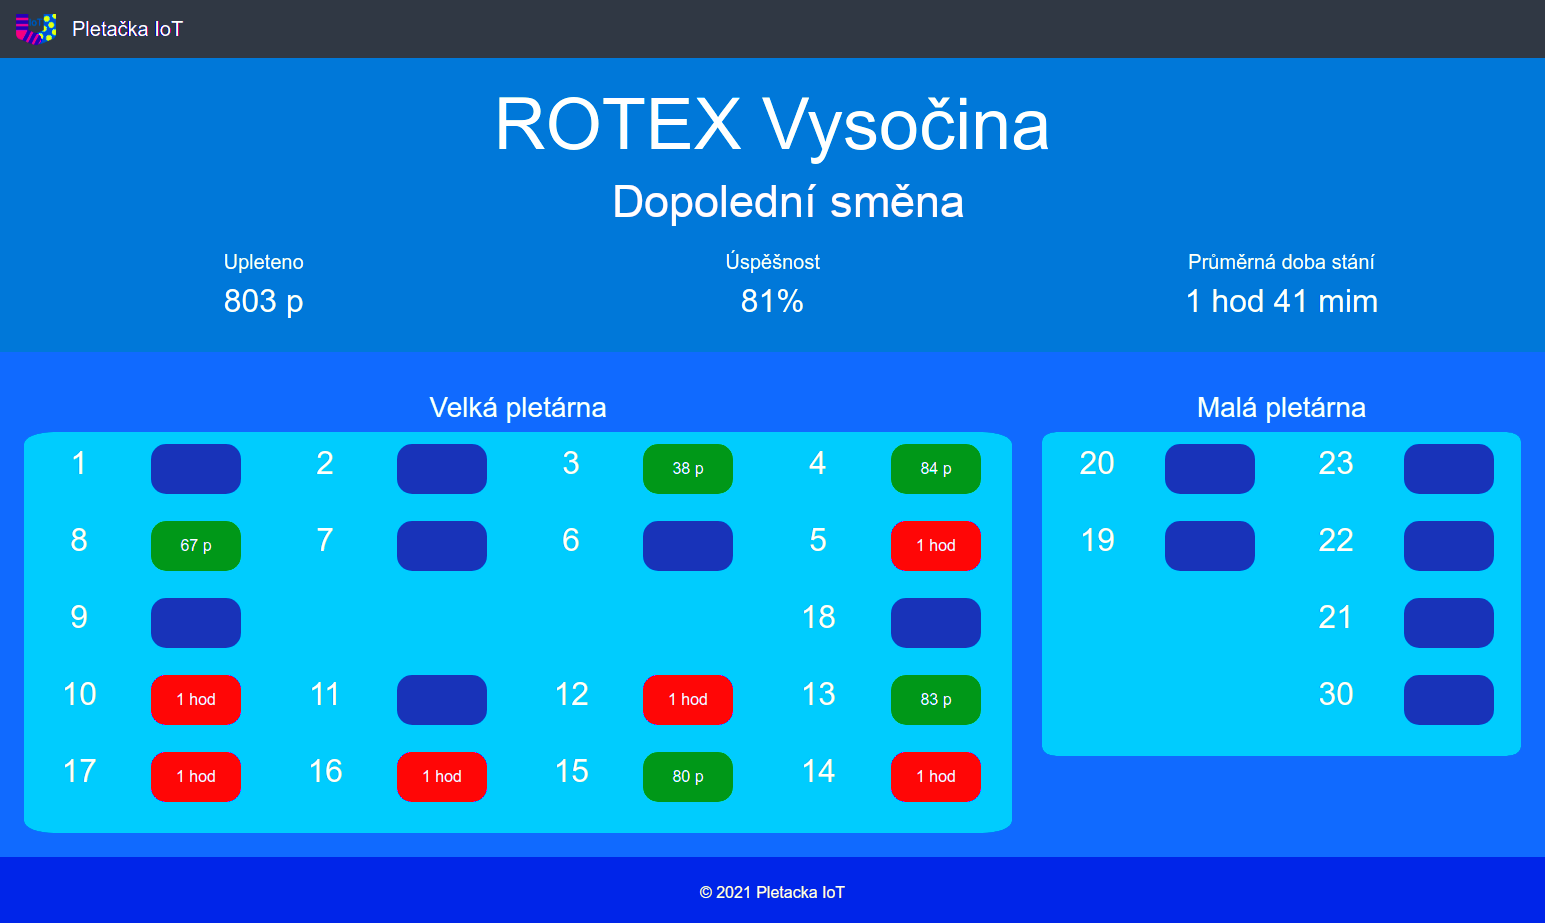
\includegraphics[width=\textwidth]{img/Uvod.png}
    \caption{Domovská stránka}
    \label{fig:webUvod}
\end{figure}

Další webovou stránkou jsou Přehledy ze senzorů generované pro každý pletací stroj.
Zde se uživateli zobrazují data v různých časových přehledech.
Pro snadné porovnání dat mezi dvěma směnami směnami se tyto údaje zobrazují vedle sebe.
Pod číselnými přehledy jsou pak předgenerované dlouhodobé grafy viz \ref{fig:webSenzory}

Každý senzor využívá pět databázových tabulek. První slouží k ukládání surových dat, do zbylých tabulek se pak ukládají automaticky generované přehledy.
Ty slouží k rychlému vykreslení grafů a výpočtu dlouhodobých údajů.
Senzor zaznamená dopletenou ponožku a skrze REST API posílá naměřený údaj na webový server, ten ji zkontroluje a uloží do databáze ke konkrétnímu senzoru.
Každý databázový záznam obsahuje číslo stroje, unikátní ID události, naměřený stav a čas události.

\begin{figure}[htbp]
    \centering
    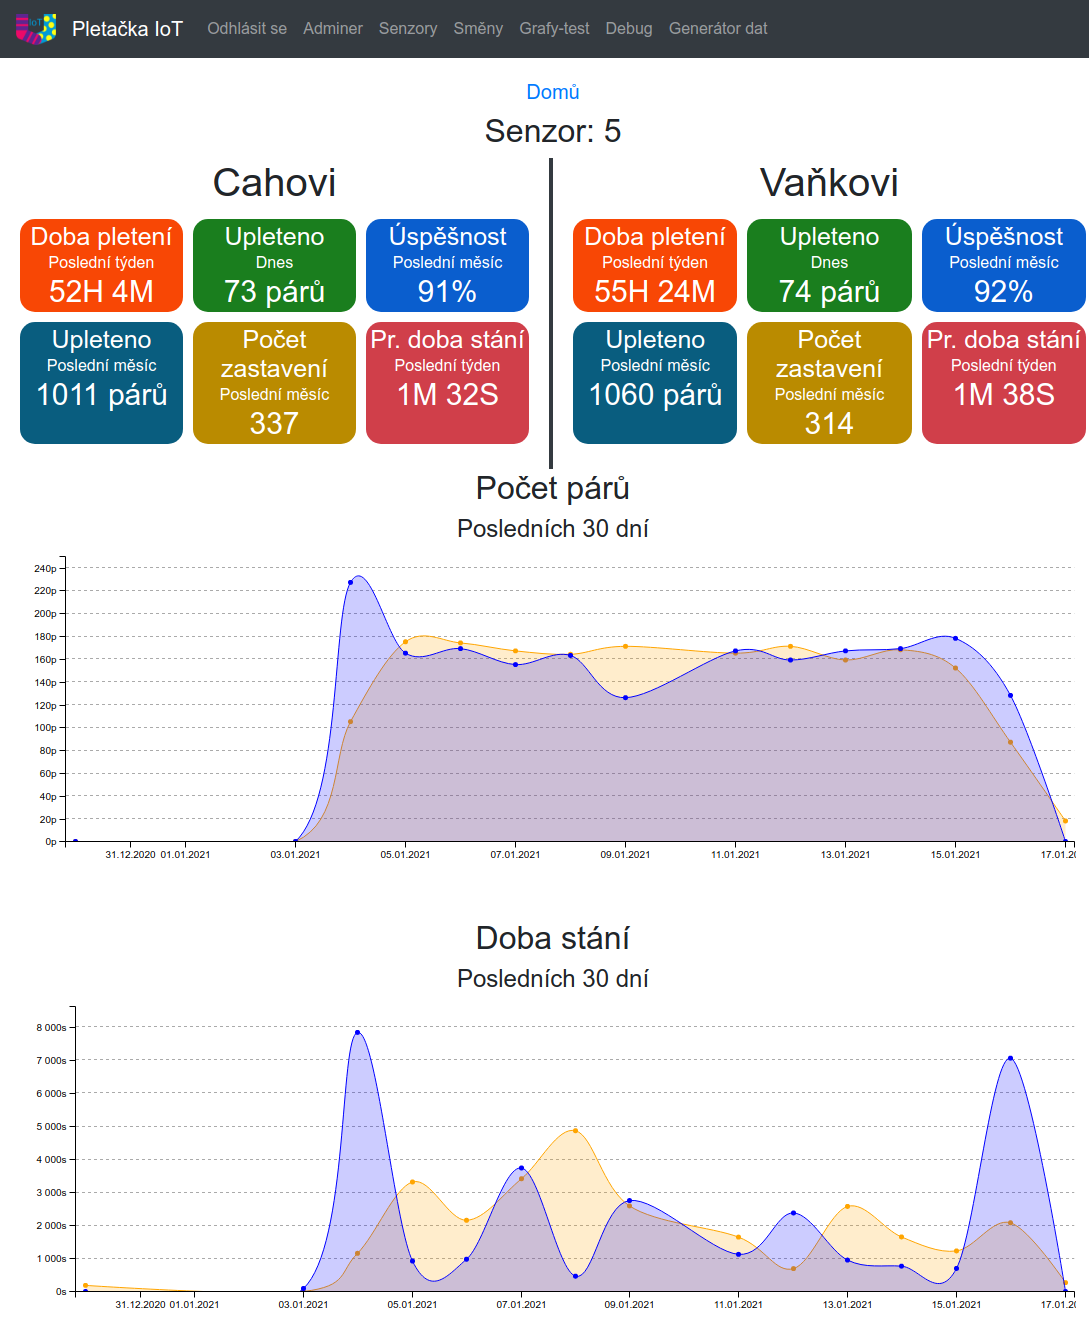
\includegraphics[width=\textwidth]{img/prehled.png}
    \caption{Přehled ze senzoru}
    \label{fig:webSenzory}
\end{figure}


% #########################################################################################
\section{Podpůrný server}
Podpůrný server vznikl jako rozšíření pro senzory.
Server je naprogramovaný v~Pythonu a~běží na Raspberry Pi společně s~webovým serverem.\newline

Hlavním úkolem tohoto serveru je detekce zapnutých senzorů.
Na serveru běží takzvaný Watchdog.
Jde o~periodickou smyčku, která každé čtyři~vteřiny čeká na zprávu ze senzoru.
Touto zprávou se senzor nahlásí, že je zapnutý. Pokud takováto zpráva nedojde do deseti vteřin, je senzor prohlášen za vypnutý a~v~databázi se označí jako neaktivní.



% #########################################################################################
\section{Princip fungování Pletačka IoT}
V~předchozích kapitolách byly popsány části systému Pletačka IoT.
V~této kapitole bude celý systém popsán jako celek.

První, a~tou nejdůležitější částí, je získávání dat pomocí senzorů.
Jakmile senzor zaznamená jakoukoliv změnu, okamžitě tuto zprávu odesílá na server.
Odesílání probíhá skrze senzorové API, kde se nejdříve senzor ověří a~následně se stav zapíše do databáze k~příslušnému senzoru.
Po zapsání do databáze se vrátí do senzoru zpráva o~provedení zápisu. 

Dalším krokem je zpracovávání surových dat z~databáze.
K~tomuto účelu běží na serveru výběrové API, které je automaticky spouštěné v~nastavený čas.
Jde o~generování širších výběrů dat, hodinové, denní, měsíční a~roční výběry.
Tyto výběry se následně ukládají do databáze k~danému senzoru.
Generování těchto dat probíhá převážně v~noci, kdy je server nejméně vytížen.

Posledním krokem je zobrazení dat uživateli.
Je to jediná část, se kterou se běžný uživatel dostane do kontaktu.
Proto je nutné, aby zobrazení bylo co nejrychlejší a~pro uživatele co nejpříjemnější.
K~rychlému zobrazování se využívají před generované výběry, ke kterým se dopočítají dosud nezpracovaná data a~celý výsledek se zobrazí uživateli.

\begin{figure}[htbp]
    \centering
    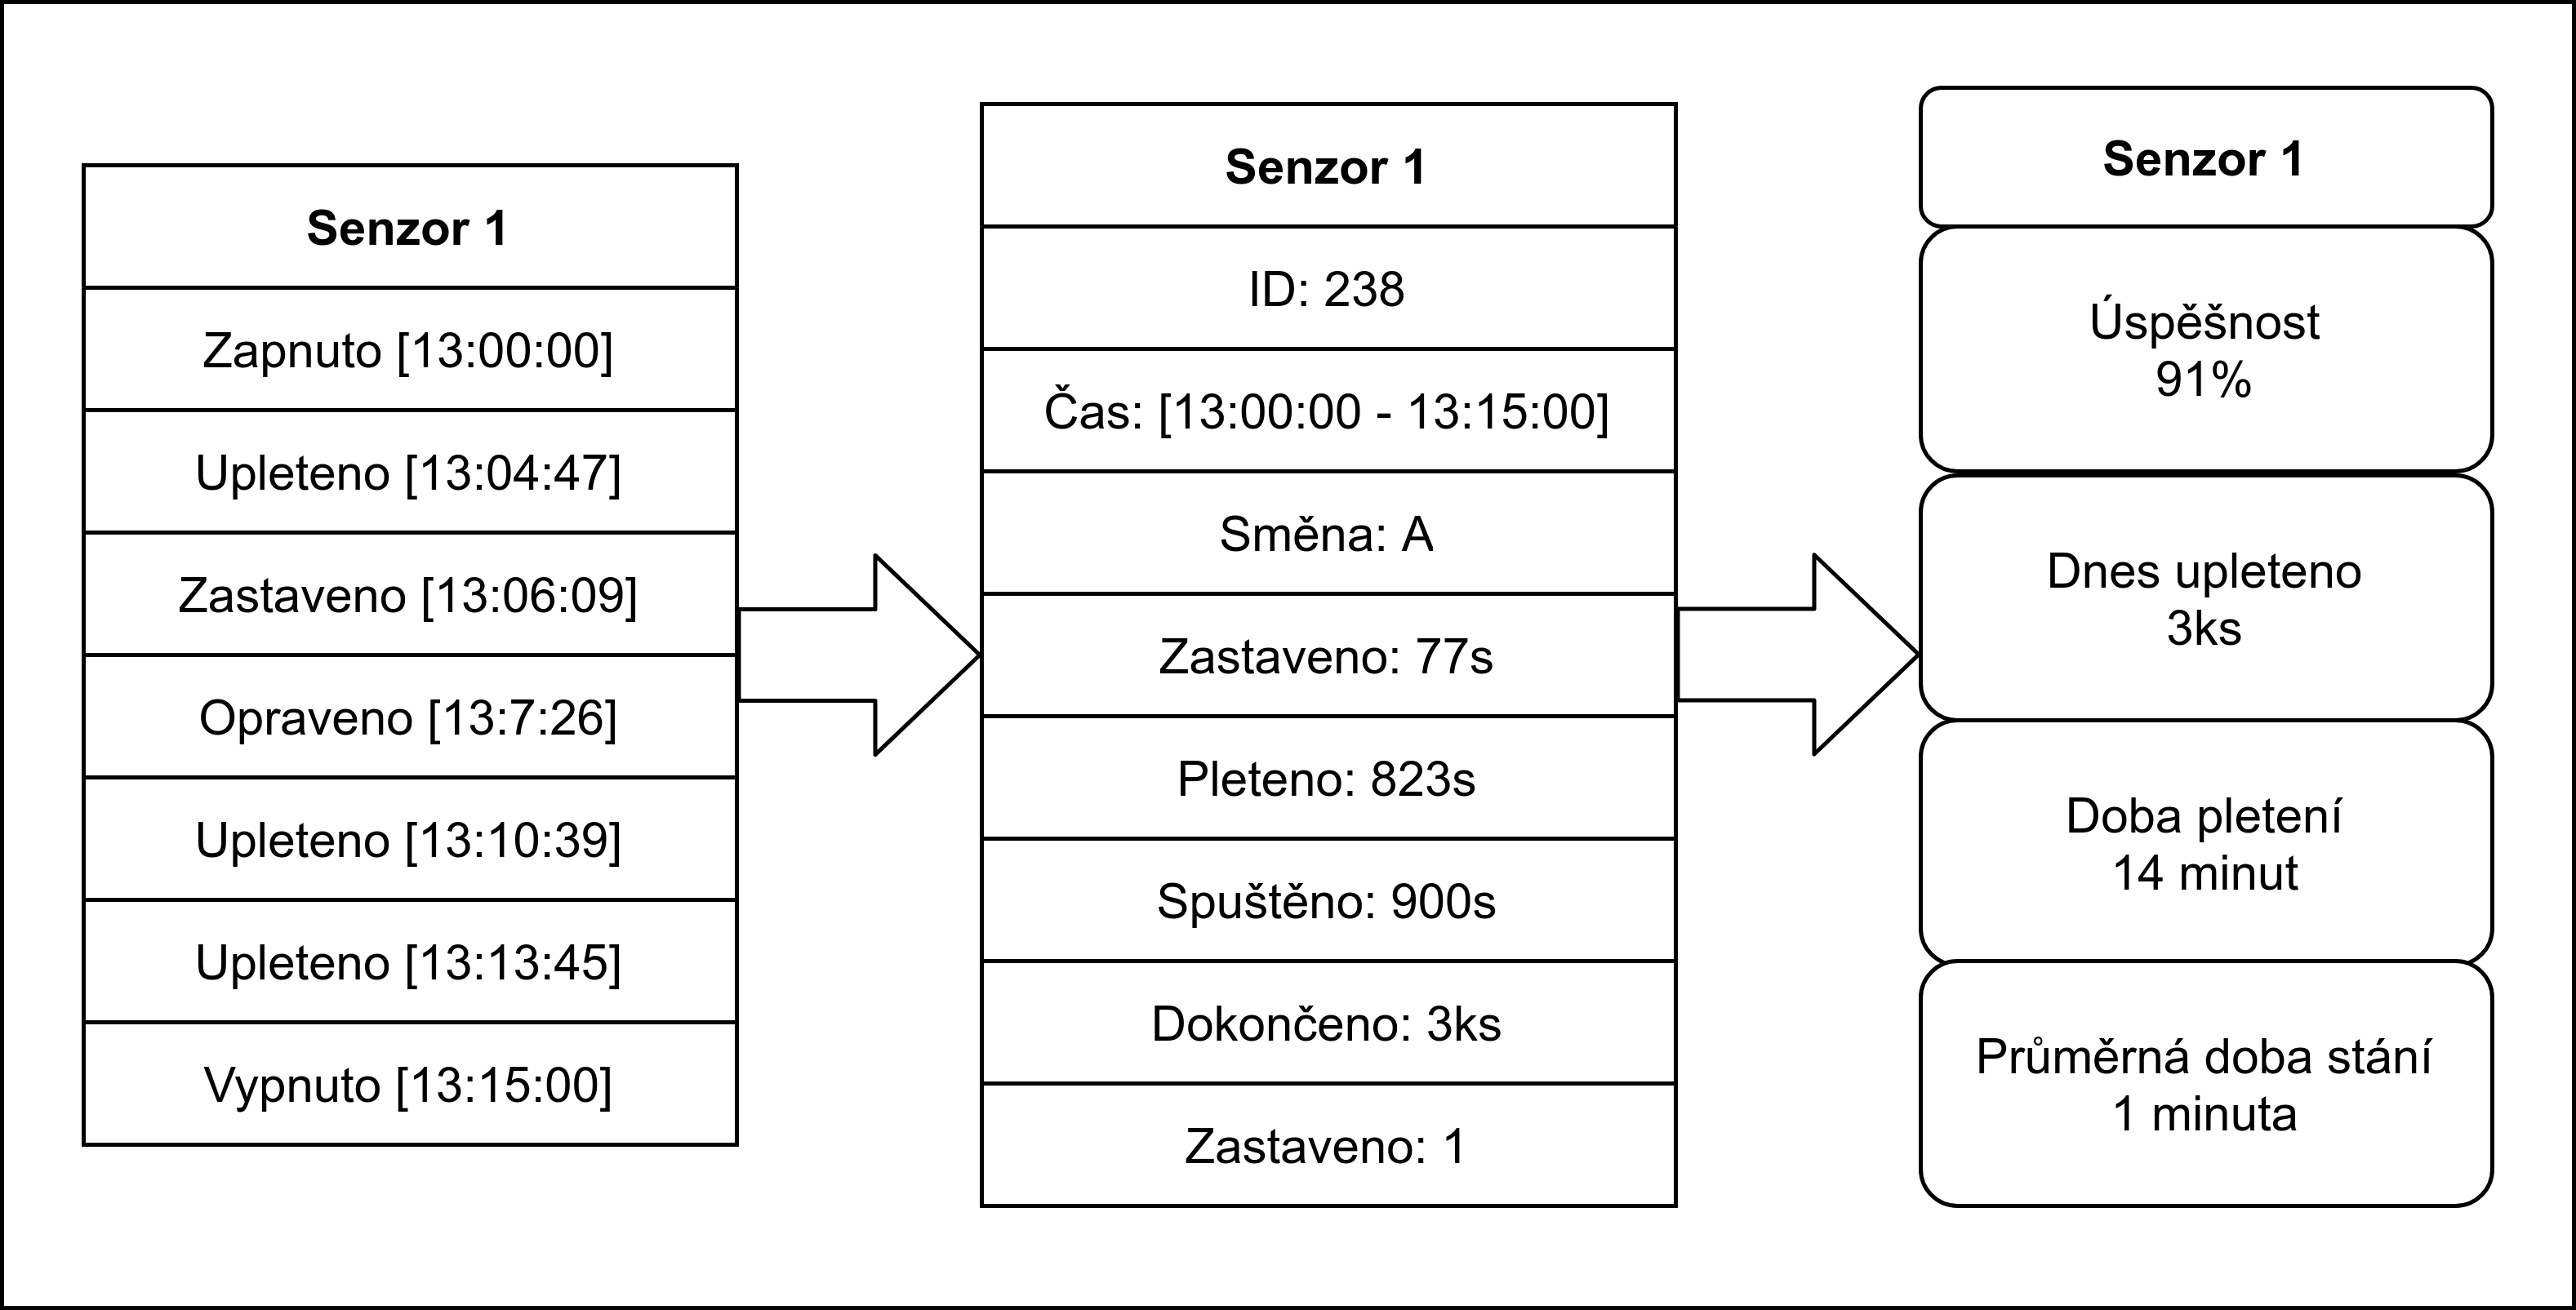
\includegraphics[width=\textwidth]{img/Princip.png}
    \caption{Zpracování dat}
    \label{fig:princip}
\end{figure}


% #########################################################################################
\section{Výsledky testování}
Celý systém jsem vyvíjel od února 2020. První testy malé testy probíhaly již od května 2020, ale k většímu nasazení došlo až v září a listopadu 2020.
Od té doby je systém ve firmě nasazen a průběžně probíhá kontrola měření a funkčnosti.

Doplním...






% #########################################################################################
\section{Závěr}

Cílem této práce bylo navrhnout ucelený systém, který dokáže:

\begin{itemize}
    \item automaticky počítat upletené ponožky
    \item on-line hlásit poruchu na stroji a~zjišťovat celkovou poruchovost strojů
    \item porovnávat výkonnost jednotlivých pracovních směn
    \item monitorovat průběh výroby
    \item nahradí část monotónní práce operátora
    \item zrychlí a~zefektivní výrobu
    \item sníží chybovost
\end{itemize}

Všechny tyto vytyčené cíle se mi podařilo splnit. Systém nadále běží ve~firmě ROTEX Vysočina s.r.o~\cite{ROTEX} a~pomáhá v~běžném provozu.
Můj systém se stal nedílnou součástí výrobního procesu a analyzuje a~zefektivňuje průběh výroby.

Systém je k 20. červnu 2021 nasazen na deseti pletacích strojích a po dobu provozu zaznamenal již přes sto padesát tisíc upletených ponožek bez závady na~senzorech.

Velkým přínosem pro firmu je porovnávání pracovních směn, díky kterým zaměstnavatel ihned vidí rozdíly mezi produktivitou práce v~daném čase.

Díky SOČ jsem se naučil navrhovat plošné spoje, rozšířil jsem si obzory v~elektronice a~při vývoji jsem si vyzkoušel práci s~měřícími přístroji. 
Také jsem se naučil programovat v~jazyce PHP a~vytvářet komplexní webové systémy.

V~budoucnu bych chtěl tento systém rozšířit na všechny pletací stroje a~pokrýt tak celou výrobu.
Taktéž pokračuji na vylepšování webové aplikace a~plánuji ji rozšířit o~další funkce.
Jde například o~export dat do tabulek.

Tuto práci můžete najít na adrese: \url{https://github.com/JakubAndrysek/SOC-Integrace-do-prumyslu-4.0/blob/master/text.pdf}.

Všechny zdrojové kódy a~DPS k~projektu jsou k~dispozici na \url{https://github.com/Pletacka-IoT} pod MIT licencí.

\newpage


\printbibliography[title=Literatura]

\addcontentsline{toc}{chapter}{Literatura}


\appendix




\end{document}

% Uprava na tvrde mezery "\b([aiouksvz]) " (i~s~tou mezerou na konci) => "$1~"
